\newpage
\section{Auswertung}
\label{sec:Auswertung}
In diesem Abschnitt werden die aufgenommenen Messdaten in Grafiken sowie Tabellen dargestellt und ausgewertet. Grafiken sowie dazugehörige Rechnungen sind mit Python \cite{python} erstellt bzw. berechnet worden.
\subsection{Stabilitätsbedingung}
\label{sec:stab}

Der Laser ist stabil, wenn Gleichung (\ref{eqn:stabi}) mit den Stabilitätsparametern aus Gleichung (\ref{eqn:g-faktor}) erfüllt ist.
Die theoretischen Kurven für die drei möglichen Spiegelanordnungen sind graphisch in Abbildung (\ref{fig:plot1}) dargestellt.
Experimentell konnte nur die Stabilitätsbedingung für Anordnung 1 und Anordnung 3 überprüft werden.
Der maximal gemessene Abstand der Resonatorspiegel beträgt für Anordnung 1 $L_\mathrm{1} = \SI{126}{\centi\meter}$ und für Anordnung 3 $L_\mathrm{3} = \SI{123}{\centi\meter}$.

\begin{figure}
  \centering
  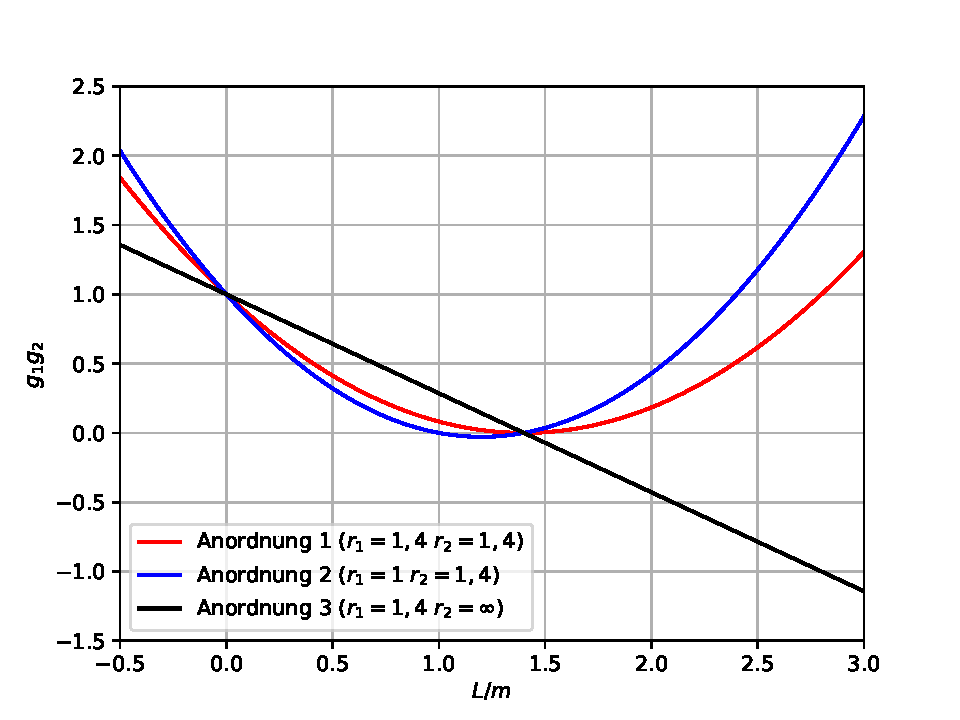
\includegraphics[scale=0.7]{fig/plot1.pdf}
  \caption{Theoretische Stabilitätsbedingungen für die drei Anordnungen.}
  \label{fig:plot1}
\end{figure}

\FloatBarrier
\subsection{Moden}
\label{sec:tem}

\subsubsection{$\mathrm{TEM}_\mathrm{00}$-Mode}

In Tabelle (\ref{tab:T00}) sind die aufgenommenen Messwerte der Grundmode $\mathrm{TEM}_\mathrm{00}$ zufinden. In Abbildung (\ref{fig:T00}) ist der Verlauf graphisch dargestellt.
Es wird aufbauend auf Gleichung (\ref{eqn:grundmode}) eine Ausgleichsrechnung der Form
\begin{equation}
  I(x) = I_\mathrm{0} \cdot \exp\left(-2\frac{(x-x_\mathrm{0})^2}{w^2}\right)
\end{equation}
durchgeführt.
Daraus ergeben sich für die Grundmode die folgenden Werte:
\begin{align*}
I_\mathrm{0} &= \SI{0.51(2)}{\micro\ampere}\\
x_\mathrm{0} &= \SI{2.89(29)}{\milli\meter}\\
w &= \SI{12.5(6)}{\milli\meter}
\end{align*}

 \begin{table}
 	\centering
 	\caption{Die gemessenen Stromstärken $I$ und die dazugehörigen Radien $r$ entlang der Horizontalen der $\mathrm{TEM}_\mathrm{00}$-Mode.}
 	\label{tab:T00}
  \begin{tabular}{c c c c}
    \toprule
    $r$ in mm & $I(r)$ in \si{\micro\ampere} & $r$ in mm & $I(r)$ in \si{\micro\ampere} \\
    \midrule
     -10 & 0,071 & 4 & 0,497 \\
     -8 & 0,101 & 6 & 0,391 \\
     -6 & 0,206 & 8 & 0,334 \\
     -4 & 0,248 & 10 & 0,283 \\
     -2 & 0,308 & 12 & 0,209 \\
     0 & 0,510 & 14 & 0,108 \\
     2 & 0,549 & 16 & 0,054 \\
    \bottomrule
  \end{tabular}
 \end{table}

\begin{figure}[h!]
  \centering
  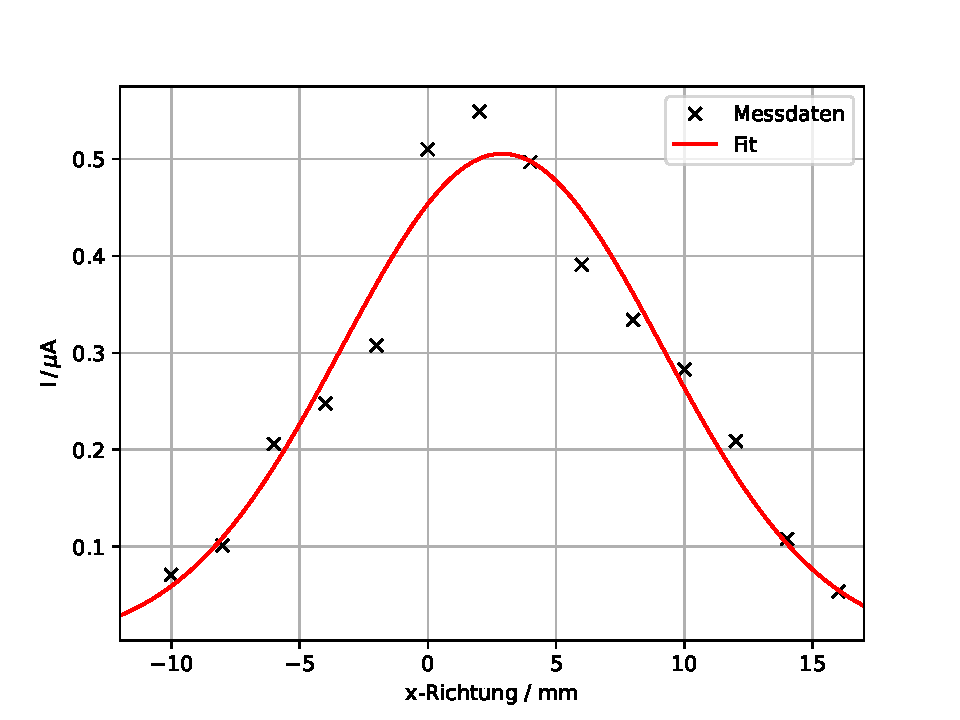
\includegraphics[scale=0.7]{fig/plot2.pdf}
  \caption{Intensitätsverteilung der $\mathrm{TEM}_\mathrm{00}$-Mode.}
  \label{fig:T00}
\end{figure}
\FloatBarrier
\subsubsection{$\mathrm{TEM}_\mathrm{01}$-Mode}

Für die $\text{TEM}_{01}$-Mode wird die Ausgleichsfunktion mit Gleichung (\ref{eqn:01}) wie folgt abgewandelt:
\begin{equation}
  I(x) = I_\mathrm{0} \cdot \dfrac{4(x-x_\mathrm{0})^2}{w^2} \cdot \exp\left(-2\frac{(x-x_\mathrm{0})^2}{w^2}\right)
\end{equation}
Die aufgenommenen Messdaten sind in Tabelle (\ref{tab:T01}) aufgelistet.
In Abbildung (\ref{fig:T01}) ist die gefittete Funktion zu sehen.
Es ergeben sich die Parameter:
\begin{align*}
I_\mathrm{0} &= \SI{0.327(9)}{\micro\ampere}\\
x_\mathrm{0} &= \SI{0.705(77)}{\milli\meter}\\
w &= \SI{6.22(11)}{\milli\meter}
\end{align*}

\begin{figure}[h!]
  \centering
  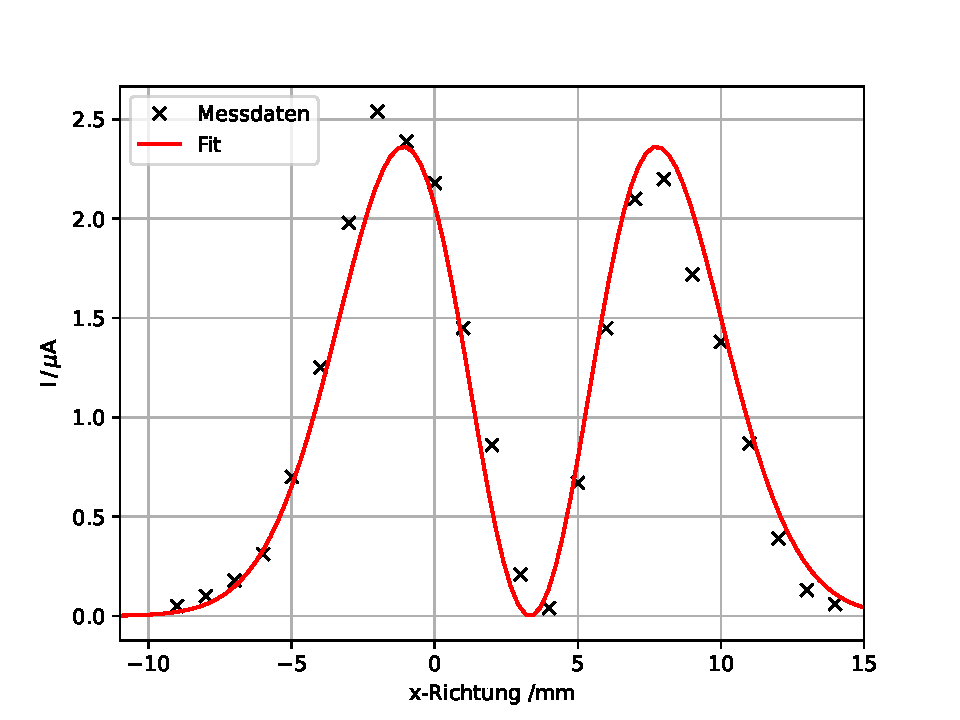
\includegraphics[scale=0.7]{fig/plot3.pdf}
  \caption{Intensitätsverteilung der $\mathrm{TEM}_\mathrm{01}$-Mode.}
  \label{fig:T01}
\end{figure}

\begin{table}
 \centering
 \caption{Die gemessenen Stromstärken $I$ und die dazugehörigen Radien $r$ entlang der Horizontalen der $\mathrm{TEM}_\mathrm{01}$-Mode.}
 \label{tab:T01}
 \begin{tabular}{c c c c}
   \toprule
   $r$ in mm & $I(r)$ in \si{\micro\ampere} & $r$ in mm & $I(r)$ in \si{\micro\ampere} \\
   \midrule
   -10 & 0,005 & 2 & 0,088 \\
   -9 & 0,012 & 3 & 0,143 \\
   -8 & 0,037 & 4 & 0,219 \\
   -7 & 0,089 & 5 & 0,239 \\
   -6 & 0,132 & 6 & 0,254 \\
   -5 & 0,174 & 7 & 0,201 \\
   -4 & 0,229  & 8 & 0,131 \\
   -3 & 0,215  & 9 & 0,069  \\
   -2 & 0,163 & 10 & 0,032 \\
   -1 & 0,065 & 11 & 0,017 \\
   0 & 0,003 & 12 & 0,009  \\
   1 & 0,023 &  &  \\
   \bottomrule
 \end{tabular}
\end{table}
\FloatBarrier
\begin{comment}
\subsubsection{$\text{TEM}_{02}$-Mode}

Zur Bestimmung der Intensitätsverteilung der $\mathrm{TEM}_\mathrm{02}$ wird die Ausgleichungsfunktion zum letzten Mal mit der Gleichung (\ref{eqn:02}) angepasst
\begin{equation}
  I(x) = I_\mathrm{0} \cdot \left(\frac{8(x-x_\mathrm{0})^2}{w^2}-2\right)^2 \cdot \exp\left(-2\frac{(x-x_\mathrm{0})^2}{w^2}\right)
\end{equation}
In Tabelle (\ref{tab:T02}) befinden sich die augenommenen Messdaten mit denen die Ausgleichsrechnung durchgeführt wird.
Diese liefert die Parameter:
\begin{align*}
I_\mathrm{0} &= \SI{0.069(4)}{\micro\ampere}\\
x_\mathrm{0} &= \SI{2.57(15)}{\milli\meter}\\
w &= \SI{6.46(16)}{\milli\meter}
\end{align*}
In Abbildung (\ref{fig:T02}) ist die gefittete Funktion dargestellt.

\begin{figure}[h!]
  \centering
  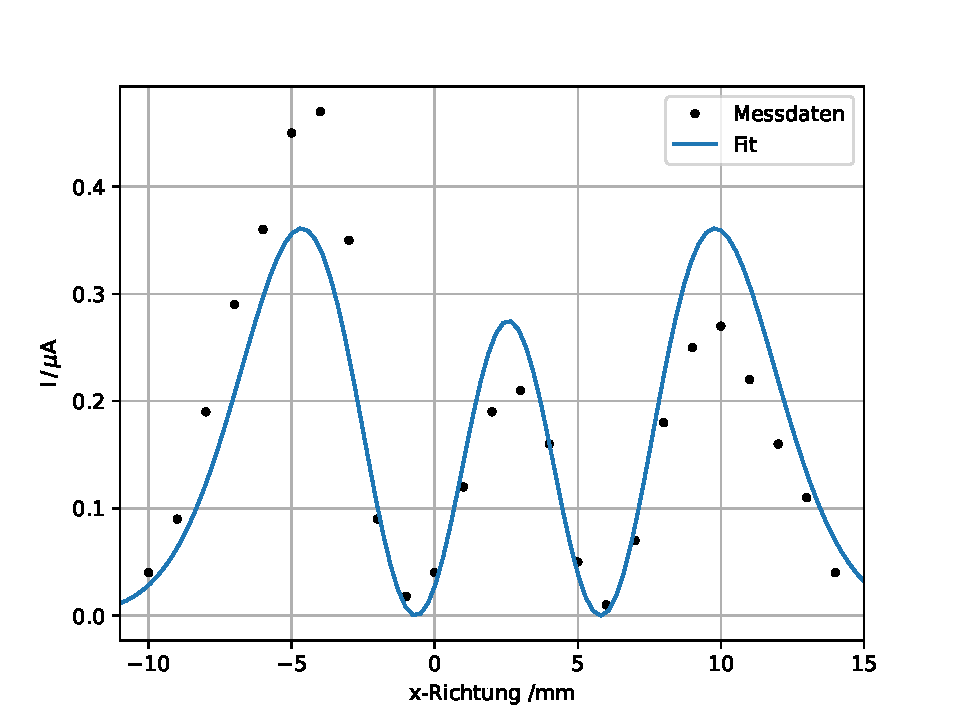
\includegraphics[scale=0.7]{fig/plot4.pdf}
  \caption{Intensitätsverteilung der $\mathrm{TEM}_\mathrm{02}$-Mode.}
  \label{fig:T02}
\end{figure}

\begin{table}
 \centering
 \caption{Die gemessenen Stromstärken $I$ und die dazugehörigen Radien $r$ entlang der Horizontalen der $\mathrm{TEM}_\mathrm{02}$-Mode.}
 \label{tab:T02}
 \begin{tabular}{c c c c}
   \toprule
   $r$ in mm & $I(r)$ in \si{\micro\ampere} & $r$ in mm & $I(r)$ in \si{\micro\ampere} \\
   \midrule
   14  & 0,04 & 1   & 0,12 \\
   13  & 0,11 & 0   & 0,04 \\
   12  & 0,16 & -1  & 0,018 \\
   11  & 0,22 & -2  & 0,09 \\
   10  & 0,27 & -3  & 0,35 \\
   9   & 0,25 & -4  & 0,47 \\
   8   & 0,18 & -5  & 0,45 \\
   7   & 0,07 & -6  & 0,36 \\
   6   & 0,01 & -7  & 0,29 \\
   5   & 0,05 & -8  & 0,19 \\
   4   & 0,16 & -9  & 0,09 \\
   3   & 0,21 & -10 & 0,04 \\
   2   & 0,19 & & \\
   \bottomrule
 \end{tabular}
\end{table}
\FloatBarrier
\end{comment}
\subsection{Polarisation}
\label{sec:pol}

In diesem Abschnitt wird nun die Polarisationsrichtung des Lasers untersucht. Wie in Abschnitt (\ref{sec:polari}) beschrieben werden die Messdaten aufgenommen.
Die Daten sind in der Tabelle (\ref{tab:polarisation}) angegeben und in Abbildung (\ref{fig:polarisation}) visualisiert.
Die gefittete Funktion hat die Form:
\begin{equation}
  I(\varphi) = I_0 \cos^2\left(\varphi+\varphi_0\right)
\end{equation}
durchgeführt.
Die dazugehörigen gefitteten Parameter lauten:
\begin{align*}
I_0 &= \SI{810.543(176)}{\nano\ampere}\\
\varphi_0 &= \SI{1.48(19)}{\radian}\\
\end{align*}

\begin{figure}[h!]
  \centering
  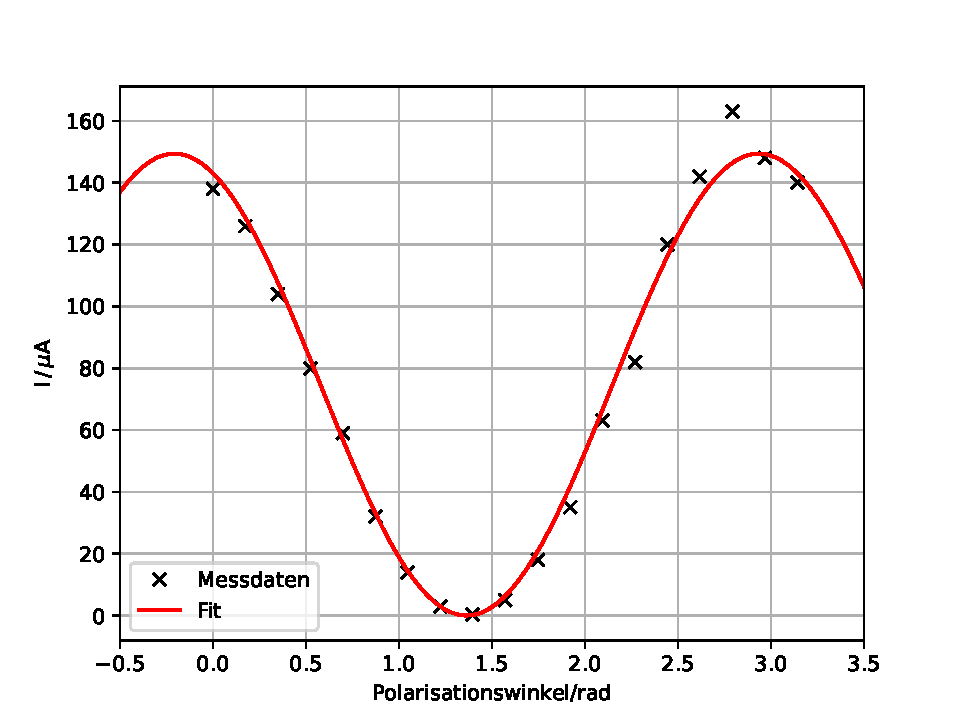
\includegraphics[scale=0.7]{fig/plot5.pdf}
  \caption{Gefittete Funktion zur Bestimmung der Polarisation des Lasers.}
  \label{fig:polarisation}
\end{figure}

\begin{table}
 \centering
 \caption{Polarisationswinkel $\varphi$ und Stromstärke $I$.}
 \label{tab:polarisation}
 \begin{tabular}{c c c c}
   \toprule
   $\varphi$ in Grad & $I(\varphi)$ in \si{\nano\ampere} & $\varphi$ in Grad & $I(\varphi)$ in \si{\nano\ampere} \\
   \midrule
   0  & 23 & 100 & 877  \\
   10 & 15 & 110 & 712 \\
   20 & 27 & 120 & 635 \\
   30 & 94  & 130 & 462  \\
   40 & 237  & 140 & 371 \\
   50 & 368 & 150 & 260 \\
   60 & 541  & 160 & 161 \\
   70 & 675   & 170 & 68 \\
   80 & 776 & 180 & 19\\
   90 & 918   & & \\
   \bottomrule
 \end{tabular}
\end{table}
\FloatBarrier
\begin{comment}
\subsection{Multimodenuntersuchung}
\label{sec:mul}

Es werden die Frequenzen $f$ der longitudinalen Moden für verschiedene Resonatorlängen vermessen und die mittlere Frequenzdifferenz $\Delta f$ berechnet.
Die Werte sind in Tabelle \ref{tab:longitudinal} eingetragen.
Theoretisch ist folgender Zusammenhang zu erwarten mit der Lichtgeschwindigkeit im Vakuum $c_0$:
\begin{equation}
  \Delta\lambda = \frac{c_0}{\Delta f} = 2L
\end{equation}
Eine Ausgleichsrechnung der Form $\Delta\lambda(L) = a \cdot L$ liefert:
\begin{equation*}
  a = \num{2.016 \pm 0.003}
\end{equation*}
Die Abhängigkeit der Frequenzdifferenzen von der Resonatorlänge ist in Abbildung \ref{fig:longitudinal} dargestellt.

\begin{table}
 \centering
 \caption{Die gemessenen Frequenzen und mittleren Frequenzdifferenzen für verschiedene Resonatorlängen.}
 \label{tab:longitudinal}
 \begin{tabular}{c c c c c c c c}
   \toprule
   $L$ in cm & \multicolumn{6}{c}{Frequenzen $f$ in MHz} & $\Delta f$ in MHz  \\
   \midrule
   87     & 173 & 341 & 510 & 683 & 851 & 1020 & 169 \\
   91     & 165 & 326 & 491 & 653 & 818 & 979  & 163 \\
   96.5   & 158 & 311 & 465 & 619 & 773 & 926  & 154 \\
   105.7  & 143 & 281 & 424 & 563 & 705 & 844  & 140 \\
   114    & 131 & 263 & 394 & 525 & 656 & 784  & 131 \\
   121.3  & 124 & 248 & 371 & 495 & 615 & 739  & 123 \\
   128    & 116 & 233 & 349 & 469 & 585 & 701  & 117 \\
   134    & 113 & 225 & 334 & 446 & 555 & 668  & 111 \\
   \bottomrule
 \end{tabular}
\end{table}

\begin{figure}
  \centering
  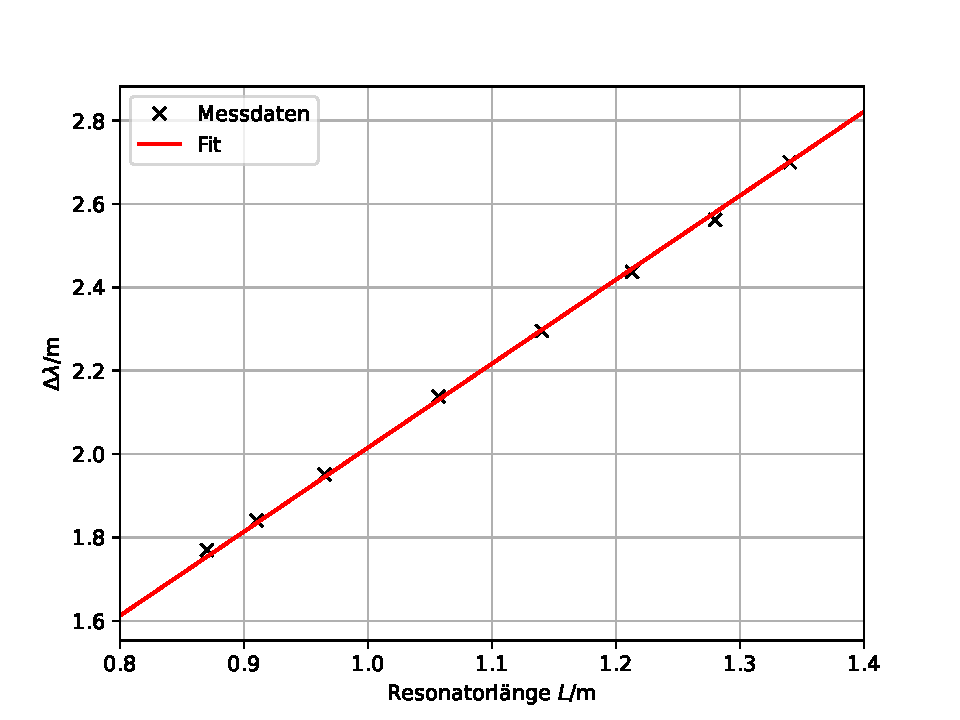
\includegraphics{fig/plot6.pdf}
  \caption{Die gemessenen Differenzen $\Delta\lambda$ in Abhängigkeit der Resonatorlänge $L$.}
  \label{fig:longitudinal}
\end{figure}

Durch den Dopplereffekt kommt es zur Verbreiterung der Spektrallinien.
Dieser Effekt wird Doppler-Verbreiterung genannt und durch die Halbwertsbreite $\delta f$ beschrieben.
\begin{equation}
  \delta f = \frac{f_0}{c} \sqrt{\frac{8 k_b T \ln(2)}{m}}
\end{equation}
Mit der Neonatommasse von $m=20,18$ u, einer Tempetatur von $T = 300$ K und für die rote Linie mit $\lambda = 632,8$ nm beträgt die Halbwertsbreite:
\begin{equation*}
  \delta f \approx \SI{1300}{MHz}
\end{equation*}
Der Laser läuft im Multimodenbetrieb, wenn die Halbwertsbreite $\delta f$ ein Vielfaches der Frequenzabstände $\Delta f$ zwischen den einzelnen Moden ist.
\end{comment}
\subsection{Wellenlänge}
\label{sec:wel}

Die Wellenlänge des Lasers kann mithilfe der Formel
\begin{equation}
  \lambda = \dfrac{\sin\left(\tan\left(\dfrac{d_n}{L}\right)\right)}{g \cdot n}
\end{equation}
bestimmt werden.
Dabei ist $d_\mathrm{n}$ der Abstand des n-ten Nebenmaxima vom Hauptmaxima, $L$ der Abstand zwischen Gitter und Schirm und $g$ die Gitterkosntante.
Die Messwerte und Ergebnisse sind in Tablle (\ref{tab:wel}) eingetragen.
Für die Wellenlänge ergibt sich so ein Mittelwert von \SI{633.845(425)}{\nano\meter}.

\begin{table}
 \centering
 \caption{Messdaten zur Messung der Wellenlänge.}
 \label{tab:wel}
 \begin{tabular}{c c c c c}
   \toprule
   Gitterkonstante $g$ & $L$ in \si{\centi\meter}  & Ordnung & Abstand $d_\mathrm{n}$ in \si{\centi\meter} & Wellenlänge $\lambda$ in \si{\nano\meter} \\
   \midrule
   100 Linien/mm & 103 & 1 & 6,5  & 631,49 \\
   100 Linien/mm & 103 & 1 & 6,6 & 641,21 \\
   80 Linien/mm & 103 & 1 & 5,2  & 631,34 \\
   80 Linien/mm & 103 & 1 & 5,2 & 631,34 \\
   \bottomrule
 \end{tabular}
\end{table}
